\documentclass[runningheads]{llncs}

% ---------------------------------------------------------------
% Include basic ACCV package
 
% TODO REVIEW: Insert your submission number below by replacing '*****'
% TODO FINAL: Comment out the following line for the camera-ready version
\usepackage[review,year=2026,ID=*****]{accv}
% TODO FINAL: Un-comment the following line for the camera-ready version
%\usepackage{accv}

% OPTIONAL: Un-comment the following line for a version which is easier to read
% on small portrait-orientation screens (e.g., mobile phones, or beside other windows)
%\usepackage[mobile]{accv}


% ---------------------------------------------------------------
% Other packages

% Commonly used abbreviations (\eg, \ie, \etc, \cf, \etal, etc.)
\usepackage{accvabbrv}

% Include other packages here, before hyperref.
\usepackage{graphicx}
\graphicspath{{content/images/report/}{content/images/drawio/}}
\usepackage{booktabs}

% The "axessiblity" package can be found at: https://ctan.org/pkg/axessibility?lang=en
% Its accsupp mode uses pdfTeX primitives that are unavailable under Tectonic's
% XeTeX engine, so load it only when those primitives exist.
\ifdefined\pdfcompresslevel
  \usepackage[accsupp]{axessibility}  % Improves PDF readability for those with disabilities.
\fi


% ---------------------------------------------------------------
% Hyperref package

% It is strongly recommended to use hyperref, especially for the review version.
% Please disable hyperref *only* if you encounter grave issues.
% hyperref with option pagebackref eases the reviewers' job, but should be disabled for the final version.
%
% If you comment hyperref and then uncomment it, you should delete
% main.aux before re-running LaTeX.
% (Or just hit 'q' on the first LaTeX run, let it finish, and you
%  should be clear).

% TODO FINAL: Comment out the following line for the camera-ready version
\usepackage[pagebackref,breaklinks,colorlinks,citecolor=accvblue]{hyperref}
% TODO FINAL: Un-comment the following line for the camera-ready version
%\usepackage{hyperref}

% Support for ORCID icon
\usepackage{orcidlink}


\begin{document}

% ---------------------------------------------------------------
% TODO REVIEW: Replace with your title
\title{Exploring Spatial and Spatio-Temporal V-JEPA 2.1 Features for Aerial Depth Estimation and Semantic Scene Completion} 

% TODO REVIEW: If the paper title is too long for the running head, you can set
% an abbreviated paper title here. If not, comment out.
% \titlerunning{Abbreviated paper title}

% TODO FINAL: Replace with your author list. 
% Include the authors' OCRID for the camera-ready version, if at all possible.
\author{First Author\inst{1}\orcidlink{0000-1111-2222-3333} \and
Second Author\inst{2,3}\orcidlink{1111-2222-3333-4444} \and
Third Author\inst{3}\orcidlink{2222--3333-4444-5555}}

% TODO FINAL: Replace with an abbreviated list of authors.
\authorrunning{F.~Author et al.}
% First names are abbreviated in the running head.
% If there are more than two authors, 'et al.' is used.

% TODO FINAL: Replace with your institution list.
\institute{Princeton University, Princeton NJ 08544, USA \and
Springer Heidelberg, Tiergartenstr.~17, 69121 Heidelberg, Germany
\email{lncs@springer.com}\\
\url{http://www.springer.com/gp/computer-science/lncs} \and
ABC Institute, Rupert-Karls-University Heidelberg, Heidelberg, Germany\\
\email{\{abc,lncs\}@uni-heidelberg.de}}

\maketitle


\begin{abstract}
  The abstract should concisely summarize the contents of the paper. 
  While there is no fixed length restriction for the abstract, it is recommended to limit your abstract to approximately 150 words.
  Please include keywords as in the example below. 
  This is required for papers in LNCS proceedings.
  \keywords{First keyword \and Second keyword \and Third keyword}
\end{abstract}


\section{Introduction}
\label{sec:introduction}

Aerial 3D scene understanding is central to autonomous uncrewed aerial vehicle (UAV) operation in cargo delivery, search and rescue, inspection, and human-UAV collaboration. In these settings, a perception system must infer not only visible image semantics, but also metric depth, free space, and the semantic occupancy of partially observed volumes. RGB cameras are attractive for UAVs because they are lightweight, inexpensive, and compatible with strict size, weight, and power constraints. However, monocular 3D perception remains difficult: image formation collapses scale, depth, and occlusion into a two-dimensional signal, and aerial views introduce altitude-dependent scale changes, oblique/top-down viewpoints, weak texture, and occlusion patterns that differ from ground-level driving scenes.

Most progress in semantic scene completion (SSC) and camera-based 3D perception has been driven by indoor and autonomous-driving benchmarks. SSCNet introduced semantic completion from depth input \cite{song2017sscnet}; MonoScene extended the task to monocular RGB \cite{cao2022monoscene}; and subsequent methods such as VoxFormer \cite{li2023voxformer}, TPVFormer \cite{huang2023tpvformer}, SurroundOcc \cite{wei2023surroundocc}, OpenOccupancy \cite{wang2023openoccupancy}, CGFormer \cite{yu2024cgformer}, and FoundationSSC \cite{chen2025foundationssc} improved view transformation, voxel attention, and semantic-geometric fusion. These designs demonstrate the value of explicit 3D representations.

OccuFly \cite{gross2026occufly} enables a focused study of this transfer problem. It provides aerial RGB images, metric depth maps, camera calibration, poses, altitude metadata, and semantic occupancy grids across multiple scenes and flight heights. Unlike 2D UAV segmentation datasets such as UAVid \cite{lyu2020uavid} or reconstruction-oriented resources such as UrbanScene3D \cite{lin2022urbanscene3d}, OccuFly supports joint evaluation of monocular depth estimation (MDE), multiview geometry, and SSC from real aerial observations. We use it to ask whether modern foundation representations provide transferable geometric and semantic priors for UAV 3D perception, and whether calibrated neighboring views improve SSC beyond monocular depth priors.

We investigate frozen V-JEPA~2.1 \cite{murlabadia2026vjepa21} image and video features for aerial MDE and depth-aware SSC. V-JEPA-style models learn by predicting latent representations rather than reconstructing pixels \cite{bardes2024vjepa,assran2025vjepa2}; V-JEPA~2.1 further emphasizes dense predictive supervision, deep self-supervision, and unified image/video tokenization. Rather than finetuning the backbone, we keep it frozen and vary only the decoder, metadata conditioning, temporal adapter, and lifting mechanism. This protocol makes the study diagnostic: improvements can be attributed to the downstream structure used to extract depth and occupancy from the representation.

Our evaluation has three parts. First, we compare linear probes, DPT-style multiscale decoders \cite{ranftl2021dpt}, Simple Feature Pyramid (SFP) adapters inspired by ViTDet \cite{li2022vitdet}, and Feature-wise Linear Modulation (FiLM) \cite{perez2018film} using altitude and camera intrinsics. This separates linear depth accessibility, dense reconstruction capacity, final-layer pyramid adaptation, and metric scale conditioning. Second, we compare RGB features with spatio-temporal V-JEPA~2.1 video features using a dense temporal-attention adapter that converts tubelet tokens into target-frame maps. Third, we evaluate SSC variants inspired by CGFormer and FoundationSSC, replacing or augmenting their geometry pathways with V-JEPA-derived depth probabilities and a pose-aware multiview stereo (MVS) cost-volume branch based on calibrated UAV views.

Our contributions are:
\begin{itemize}
    \item A systematic frozen-backbone evaluation of V-JEPA~2.1 RGB and video representations for aerial metric depth estimation on OccuFly.
    \item A controlled comparison of linear probes, DPT-style decoders, SFP-adapted final-layer decoders, and altitude/intrinsics-conditioned FiLM variants.
    \item An analysis of spatio-temporal feature transfer through dense temporal attention over V-JEPA~2.1 video tokens.
    \item A depth-to-SSC study that injects V-JEPA-derived depth maps and depth distributions into CGFormer- and FoundationSSC-inspired aerial SSC variants.
    \item A pose-aware FoundationSSC variant that replaces monocular depth lifting with calibrated multiview cost-volume depth estimation from neighboring UAV frames.
\end{itemize}

\section{Related Work}

Write the related work for the target conference paper.

\section{Method}

Write the method for the target conference paper.

\section{Experimental Setup}
\label{sec:blind}
ACCV reviewing is double blind, in that authors do not know the names of the Area Chairs or reviewers of their papers, and Area Chairs and reviewers should not, beyond reasonable doubt, be able to infer the identities of the authors from the submission or supplementary material.
You must not identify the authors in the paper or supplementary material. External links must not be used to expand the content under review or to provide material that should instead be included directly in the submission or supplementary files. Code, videos, images, and other media intended for review may be submitted in anonymized form as supplementary material, but should not be provided through external links.
If you need to cite a different paper of yours that is being submitted concurrently to ACCV, you should \emph{(1)} cite these papers anonymously, \emph{(2)} explain in the body of your paper why your ACCV paper is non-trivially different from these concurrent submissions, and \emph{(3)} include anonymized versions of those papers in the supplementary material.
Violation of any of these guidelines may lead to rejection without review.

Many authors misunderstand the concept of anonymizing for blind review.
Blind review does not mean that one must remove citations to one's own work---in fact it is often impossible to review a paper unless the previous citations are known and available.

Blind review means that you do not use the words ``my'' or ``our'' when citing previous work.
That is all.
(But see below for tech reports.)

Saying ``this builds on the work of Lucy Smith [1]'' does not say that you are Lucy Smith;
it says that you are building on her work.
If you are Smith and Jones, do not say ``as we show in [7]'', say ``as Smith and Jones show in [7]'' and at the end of the paper, include reference 7 as you would any other cited work.

An example of a bad paper just asking to be rejected:
\begin{quote}
  \begin{center}
      An analysis of the frobnicatable foo filter.
  \end{center}

   In this paper we present a performance analysis of our previous paper [1], and show it to be inferior to all previously known methods.
   Why the previous paper was accepted without this analysis is beyond me.

   [1] Removed for blind review
\end{quote}

An example of an acceptable paper:
\begin{quote}
  \begin{center}
     An analysis of the frobnicatable foo filter.
  \end{center}

   In this paper we present a performance analysis of the  paper of Smith \etal [1], and show it to be inferior to all previously known methods.
   Why the previous paper was accepted without this analysis is beyond me.

   [1] Smith, L and Jones, C. ``The frobnicatable foo filter, a fundamental contribution to human knowledge''. Nature 381(12), 1-213.
\end{quote}

If you are making a submission to another conference at the same time, which covers similar or overlapping material, you may need to refer to that submission in order to explain the differences, just as you would if you had previously published related work.
In such cases, include the anonymized parallel submission [1] as supplemental material and cite it as
\begin{quote}
  [1] Authors. ``The frobnicatable foo filter'', ACCV \ACCVyear Submission ID 00324, Supplied as supplemental material {\tt 00324.pdf}.
\end{quote}

Finally, you may feel the need to indicate that additional details exist elsewhere, such as in a technical report.
For conference submissions, however, the paper must stand on its own and must not require reviewers to consult outside material in order to evaluate the submission.
If additional supporting material is necessary, it should be provided in anonymized form as supplementary material rather than through an external link.
Again, you may not assume that reviewers will read supplementary material.

Sometimes your paper is about a problem, which you tested using a tool that is widely known to be restricted to a single institution.
For example, let's say it's 1969, you have solved a key problem on the Apollo lander, and you believe that the ACCV audience would like to hear about your
solution.
The work is a development of your celebrated 1968 paper entitled ``Zero-g frobnication: How being the only people in the world with access to the Apollo lander source code makes us a wow at parties'', by Zeus \etal.

You can handle this paper like any other.
Do not write ``We show how to improve our previous work [Anonymous, 1968].
This time we tested the algorithm on a lunar lander [name of lander removed for blind review]''.
That would be silly, and would immediately identify the authors.
Instead write the following:
\begin{quotation}
   We describe a system for zero-g frobnication.
   This system is new because it handles the following cases:
   A, B.  Previous systems [Zeus et al. 1968] did not  handle case B properly.
   Ours handles it by including a foo term in the bar integral.

   ...

   The proposed system was integrated with the Apollo lunar lander, and went all the way to the moon, don't you know.
   It displayed the following behaviours, which show how well we solved cases A and B: ...
\end{quotation}
As you can see, the above text follows standard scientific convention, reads better than the first version, and does not explicitly name you as the authors.
A reviewer might think it likely that the new paper was written by Zeus \etal, but cannot make any decision based on that guess.
He or she would have to be sure that no other authors could have been contracted to solve problem B.

For sake of anonymity, authors must omit acknowledgements in the review copy. 
They can be added later when you prepare the final copy.


\section{Results and Discussion}

\subsection{Headings}
Headings should be capitalized (\ie, nouns, verbs, and all other words except articles, prepositions, and conjunctions should be set with an initial capital) and should, with the exception of the title, be aligned to the left.
Only the first two levels of section headings should be numbered, as shown in \cref{tab:headings}.
The respective font sizes are also given in \cref{tab:headings}. 
Kindly refrain from using ``0'' when numbering your section headings.
Words joined by a hyphen are subject to a special rule. 
If the first word can stand alone, the second word should be capitalized.

\begin{table}[tb]
  \caption{Font sizes of headings. 
    Table captions should always be positioned \emph{above} the tables.
  }
  \label{tab:headings}
  \centering
  \begin{tabular}{@{}lll@{}}
    \toprule
    Heading level & Example & Font size and style\\
    \midrule
    Title (centered)  & {\Large\bf Lecture Notes \dots} & 14 point, bold\\
    1st-level heading & {\large\bf 1 Introduction} & 12 point, bold\\
    2nd-level heading & {\bf 2.1 Printing Area} & 10 point, bold\\
    3rd-level heading & {\bf Headings.} Text follows \dots & 10 point, bold\\
    4th-level heading & {\it Remark.} Text follows \dots & 10 point, italic\\
  \bottomrule
  \end{tabular}
\end{table}

Here are some examples of headings: 
``Criteria to Disprove Context-Freeness of Collage Languages'', ``On Correcting the Intrusion of Tracing Non-deterministic Programs by Software'', ``A User-Friendly and Extendable Data Distribution System'', ``Multi-flip Networks: Parallelizing GenSAT'', ``Self-determinations of Man''.


\subsection{Figures}
\label{sect:figures}
For \LaTeX{} users, we recommend integrating figures in your paper using the package \texttt{graphicx}.

It is essential that all illustrations are clear and legible. 
Vector graphics (rather than rasterized images) should be used for diagrams and schemas whenever possible. 
Please check that the lines in line drawings are not interrupted and have a constant width. 
Line drawings are to have a resolution of at least 800 dpi (preferably 1200 dpi).
Grids and details within figures must be clearly legible and may not be written one on top of the other. 
The lettering in figures should not use font sizes smaller than 6\:pt ($\sim$2\:mm character height). 

Figures should be numbered and should have a caption, which should always be positioned \emph{under} the figures, in contrast to the caption belonging to a table, which should always appear \emph{above} the table.
Figures and Tables should be cross-referred in the text.

If they are short, they are centered between the margins (\cf \cref{fig:short}). 
Longer captions, covering more than one line, are justified (\cref{fig:example} shows an example). 
Captions that do not constitute a full sentence, do not have a period.


\begin{figure}[tb]
  \centering
  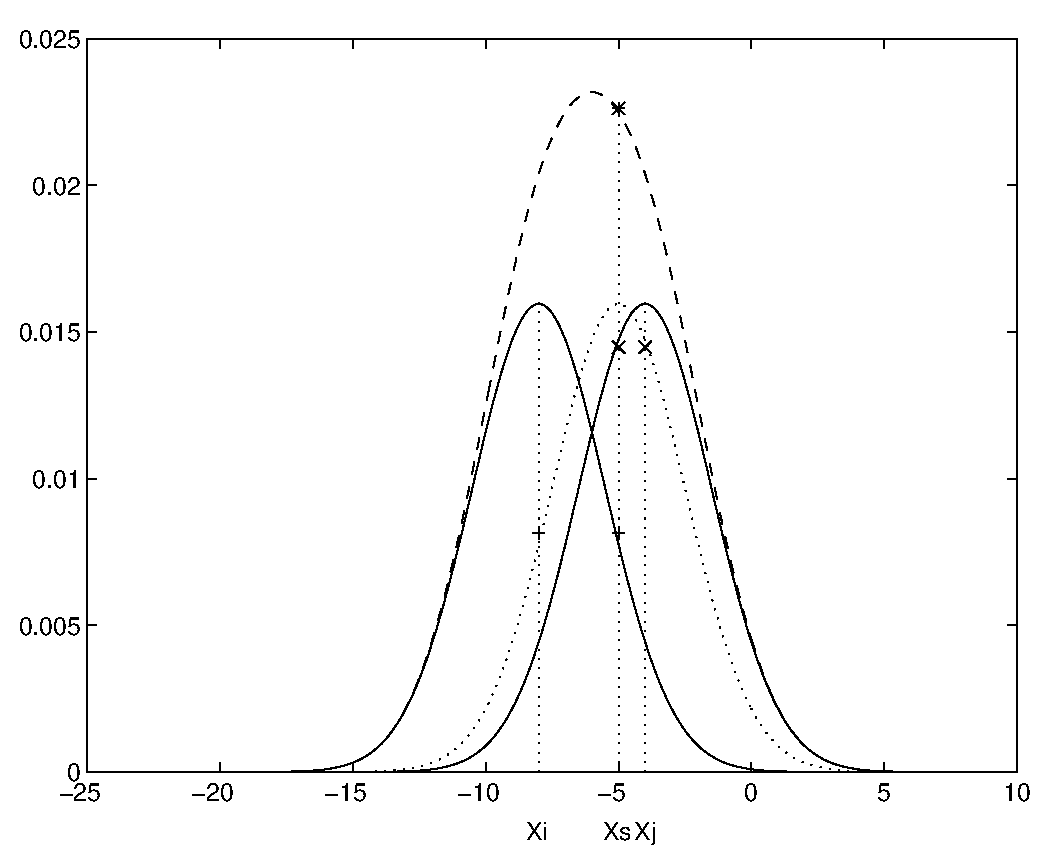
\includegraphics[height=6.5cm]{eijkel2}
  \caption{One kernel at $x_s$ (\emph{dotted kernel}) or two kernels at $x_i$ and $x_j$ (\emph{left and right}) lead to the same summed estimate at $x_s$.
    This shows a figure consisting of different types of lines.
    Elements of the figure described in the caption should be set in italics, in parentheses, as shown in this sample caption. 
    The last sentence of a figure caption should generally end with a full stop, except when the caption is not a full sentence.
  }
  \label{fig:example}
\end{figure}

\begin{figure}[tb]
  \centering
  \begin{subfigure}{0.68\linewidth}
    \fbox{\rule{0pt}{0.5in} \rule{.9\linewidth}{0pt}}
    \caption{An example of a subfigure}
    \label{fig:short-a}
  \end{subfigure}
  \hfill
  \begin{subfigure}{0.28\linewidth}
    \fbox{\rule{0pt}{0.5in} \rule{.9\linewidth}{0pt}}
    \caption{Another example of a subfigure}
    \label{fig:short-b}
  \end{subfigure}
  \caption{Centered, short example caption}
  \label{fig:short}
\end{figure}

If possible (\eg, if you use \LaTeX) please define figures as floating objects. 
\LaTeX{} users, please avoid using the location parameter ``h'' for ``here''. 
If you have to insert a pagebreak before a figure, please ensure that the previous page is completely filled.


\subsection{Formulas}
Displayed equations or formulas are centered and set on a separate line (with an extra line or half line space above and below). 
Equations should be numbered for reference. 
The numbers should be consecutive within the contribution, with numbers enclosed in parentheses and set on the right margin.
For example,
\begin{align}
  \psi (u) & = \int_{0}^{T} \left[\frac{1}{2}
  \left(\Lambda_{0}^{-1} u,u\right) + N^{\ast} (-u)\right] \text{d}t \; \\
& = 0
\end{align}
and 
\begin{equation}
  E = m\cdot c^2.
  \label{eq:important}
\end{equation}
Please do not include section counters in the numbering.

Numbering equations makes reviewing more efficient, because reviewers can refer to a line on a page.  
It is important for readers to be able to refer to any particular equation.
Just because you did not refer to it in the text does not mean some future reader might not need to refer to it.
It is cumbersome to have to use circumlocutions like ``the equation second from the top of page 3''.
(Note that the ruler will not be present in the final copy, so is not an alternative to equation numbers).
All authors will benefit from reading Mermin's description of how to write mathematics:
\url{https://doi.org/10.1063/1.2811173}.

% No color equations in Springer publications.
Equations should never be in color and should be punctuated in the same way as ordinary text.
They should not be pasted in as figures.


\subsubsection{Lemmas, Propositions, and Theorems.}
The numbers accorded to lemmas, propositions, and theorems, \etc should appear in consecutive order, starting with Lemma 1. 
Please do not include section counters in the numbering like ``Theorem 1.1''.


\subsection{Footnotes.}
The superscript numeral used to refer to a footnote appears in the text either directly after the word to be discussed or -- in relation to a phrase or a sentence -- following the punctuation mark (comma, semicolon, or period).%
\footnote{The footnote numeral is set flush left and the text follows with the usual word spacing. 
  Second and subsequent lines are indented. 
}
For remarks pertaining to the title or the authors' names, in the header of a paper, symbols should be used instead of a number.
Please note that no footnotes may be included in the abstract.


\subsection{Cross References}
For the benefit of author(s) and readers, please use the
\begin{verbatim}
  \cref{...}
\end{verbatim}
command for cross-referencing to figures, tables, equations, or sections.
This will automatically insert the appropriate label alongside the cross reference as in this example:
\begin{quotation}
  To see how our method outperforms previous work, please see \cref{fig:example} and \cref{tab:headings}.
  It is also possible to refer to multiple targets as once, \eg~to \cref{fig:example,fig:short-a}.
  You may also return to \cref{sec:intro} or look at \cref{eq:important}.
\end{quotation}
If you do not wish to abbreviate the label, for example at the beginning of the sentence, you can use the
\begin{verbatim}
  \Cref{...}
\end{verbatim}
command. Here is an example:
\begin{quotation}
  \Cref{fig:example} is also quite important.
\end{quotation}


\subsection{Program Code}
Program listings or program commands in the text are normally set in typewriter font (\eg, \texttt{printf("Hello world!\textbackslash{}n");}).


\subsection{Citations}
Arabic numbers are used for citation, which is sequential either by order of citation or by alphabetical order of the references, depending on which sequence is used in the list of references. 
The reference numbers are given in brackets and are not superscript.
Please observe the following guidelines:
\begin{itemize}
\item Single citation: \cite{Anonymous24}
\item Multiple citation: \cite{Alpher02,Alpher03,Alpher05,Anonymous24b,Anonymous24}. 
  The numbers should be listed in numerical order.
  If you use the template as advised, this will be taken care of automatically.
\item If an author's name is used in the text: Alpher \cite{Alpher02} was the first \ldots
\end{itemize}
Please write all references using the Latin alphabet. If the title of the book you are referring to is, \eg, in Russian or Chinese, then please write (in Russian) or (in Chinese) at the end of the transcript or translation of the title.
All references cited in the text should be in the list of references and vice versa.

References should be formatted with the official LNCS reference style.
The \LaTeX{} template already takes care of that through the use of the \texttt{splncs04.bst} Bib\TeX{} style file.
Springer strongly encourages you to include DOIs (Digital Object Identifiers) in your references (\cf \cite{ECCV2022}). 
The DOI is a unique code allotted by the publisher to each online paper or journal article. 
It provides a stable way of finding published papers and their metadata. 
The insertion of DOIs increases the overall length of the references section, but this should not concern you as the reference section is not counted toward the page limit.


\subsection{Miscellaneous}
Compare the following:
\begin{center}
  \begin{tabular}{ll}
    \verb'$conf_a$'          & $\qquad conf_a$ \\
    \verb'$\mathit{conf}_a$' & $\qquad \mathit{conf}_a$
  \end{tabular}
\end{center}
See The \TeX book, p.\ 165.

The space after \eg, meaning ``for example'', should not be a sentence-ending space.
So \eg is correct, \emph{e.g.} is not.
The provided \verb'\eg' macro takes care of this.

When citing a multi-author paper, you may save space by using ``et alia'', 
shortened to ``\etal'' (not ``{\em et.\ al.}'' as ``{\em et\hskip 0.1em}'' is a complete word).
If you use the \verb'\etal' macro provided, then you need not worry about double periods when used at the end of a sentence as in Alpher \etal.
However, use it only when there are three or more authors.
Thus, the following is correct:
   ``Frobnication has been trendy lately.
   It was introduced by Alpher~\cite{Alpher02}, and subsequently developed by
   Alpher and Fotheringham-Smythe~\cite{Alpher03}, and Alpher \etal~\cite{Alpher04}.''

This is incorrect: ``... subsequently developed by Alpher \etal~\cite{Alpher03} ...'' because reference~\cite{Alpher03} has just two authors.


\section{Conclusion}
The paper ends with a conclusion. 

\subsection{Camera-Ready Manuscript Preparation}
\label{sec:manuscript}
This information will follow after paper decisions have been announced.

\clearpage\mbox{}Page \thepage\ of the manuscript.
\clearpage\mbox{}Page \thepage\ of the manuscript.
\clearpage\mbox{}Page \thepage\ of the manuscript.
\clearpage\mbox{}Page \thepage\ of the manuscript.
\clearpage\mbox{}Page \thepage\ of the manuscript. This is the last page.
\par\vfill\par
Now we have reached the maximum length of an ACCV \ACCVyear{} submission (excluding references).
References should start immediately after the main text, but can continue past p.\ 14 if needed.
\clearpage  % TODO REVIEW/FINAL: This \clearpage needs to be removed from both review and camera-ready versions.


% ---- Bibliography ----
%
% BibTeX users should specify bibliography style 'splncs04'.
% References will then be sorted and formatted in the correct style.
%
\bibliographystyle{splncs04}
\bibliography{content/references}
\end{document}
